%% LyX 2.2.3 created this file.  For more info, see http://www.lyx.org/.
%% Do not edit unless you really know what you are doing.
\documentclass[english,aps,preprint,nofootinbib]{revtex4}
\usepackage[T1]{fontenc}
\usepackage[latin9]{inputenc}
\usepackage{amssymb}
\usepackage{bbm}

\usepackage{amsmath}
\setcounter{secnumdepth}{3}

\makeatletter
%%%%%%%%%%%%%%%%%%%%%%%%%%%%%% Textclass specific LaTeX commands.
\@ifundefined{textcolor}{}
{%
 \definecolor{BLACK}{gray}{0}
 \definecolor{WHITE}{gray}{1}
 \definecolor{RED}{rgb}{1,0,0}
 \definecolor{GREEN}{rgb}{0,1,0}
 \definecolor{BLUE}{rgb}{0,0,1}
 \definecolor{CYAN}{cmyk}{1,0,0,0}
 \definecolor{MAGENTA}{cmyk}{0,1,0,0}
 \definecolor{YELLOW}{cmyk}{0,0,1,0}
}

\makeatother
\usepackage{amsthm}

\usepackage{babel}
\usepackage{graphicx}
\usepackage{caption}
\usepackage{subfig}


\begin{document}

\title{\noindent Optimal Service Elasticity in Large-Scale Distributed Systems }

\author{\noindent Debankur Mukherjee et al.}

\affiliation{\noindent Eindhoven University of Technology}

\author{\noindent Analysis by Noah Johnson}

\affiliation{\noindent College of Electrical Computer and Biomedical Engineering, University of Rhode Island}


\maketitle
\tableofcontents
\pagebreak
\section{introduction}

\noindent Latency in server systems can be extremely detrimental on
an end user's experience. In banking systems, for example, even a
few milliseconds of delay can be catastrophic. However, where the
bottleneck was once lack of resources due to underpowered hardware
and prohibitive cost, this has changed in recent years. The bottleneck
is now maximizing allocation of server resources while minimizing
energy usage. This is, of course, a hard problem with no clear solution.
In their paper, "Optimal Service Elasticity in Large-Scale Distributed
Systems" Mukherjee et al. present a novel scheme for automatic load-balancing
between individual servers in a large scale system. This scheme utilizes
constant overhead for control messages per task in the system, and
requires no global queue information, a common requirement in many
noteworthy schema of the same type. They demonstrate that the scheme
provides provably near-optimal task waiting time and energy wastage
measures for large server farms. They further prove that the scheme
provides optimal results in the limit as the number of servers tends
to infinity, and that these results extend from traditional arrival
distributions to phase-type distributions.

\section{The Problem}

\noindent As the complexity and overall size of distributed computing
systems increases, the power loss and latency of the system become
much more of a problem than the service resources available. This
is the premise of service elasticity as defined in the paper. The
problem is then as follows:

\begin{quote}
    \textbf{How do we dynamically scale the available server
        resources with the observed load conditions, while maintaining minimal
        energy loss from idle servers and satisfying several performance criteria?}
\end{quote}

\noindent This is a difficult problem to solve, as turning servers
on to meet a changing arrival process takes some amount of time, and
thus the server resources available will always lag behind the needs
of the observed system load, usually by an amount far exceeding acceptable
system latency limits. However this is only true if the reactive balancing
method used is naive. Generally, predictive models are preferred, and will
yield better results, with several serious caveats. Typically, these schema
require a centralized queue, which is not generally true in distributed
computing systems. In addition, maintaining such a queue would entail
significant, often prohibitive, computational overhead. So how do we
efficiently balance incoming load on a distributed system in a strictly
reactive manner, while maintaining First-Come-First-Serve policy at each of the servers?

\section{TABS Algorithm Explanation}

\noindent Mukherjee et al. propose the following scheme, called "Token-based Auto Balance
Scaling", or TABS. The most basic part of TABS is that given a distributed system, each
server has a colored token, which it uses to tell a job dispatcher about its current state. The token can be one of 4 colors:

\begin{enumerate}
    \item[\textbf{Red}] - Denoting that the server is in the "idle-off" state.
    \item[\textbf{Green}] - Denoting that the server is in the "idle-on" state and is ready to accept jobs.
    \item[\textbf{Yellow}] - Denoting that the server is "busy" (i.e. it has at least one job allocated to it, including the one it is working on.)
    \item[\textbf{Orange}] - Denoting that the server is currently in "setup" mode, and cannot accept any jobs.
\end{enumerate}

\noindent The servers in the system turn on and off according to several rules. When a server becomes idle, it sends
a "green" (idle-on) message to the dispatcher, and enters the idle-on period, where it will stay for a period of
time $t_{idle}$ which follows the distribution $t_{idle} \sim Exp(\mu_{idle})$. If, after $t_{idle}$ time units
have passed and the server has received no new jobs, then it will shut itself off, and send a "red" (idle-off) message to the dispatcher.
When a job arrives in the system, then the dispatcher will immediately look for a green server to send the job to (recall that the main
goal of TABS is to minimize waiting time. A green server will have zero jobs queued, and thus any new job will experience zero waiting time).
At this point the server in question will send a "yellow" message to the dispatcher, and will stay in the busy state until it has finished all
of the jobs in its queue. Note that yellow servers \textit{can} accept new jobs from the dispatcher.

\begin{figure*}[h]
    \centering
    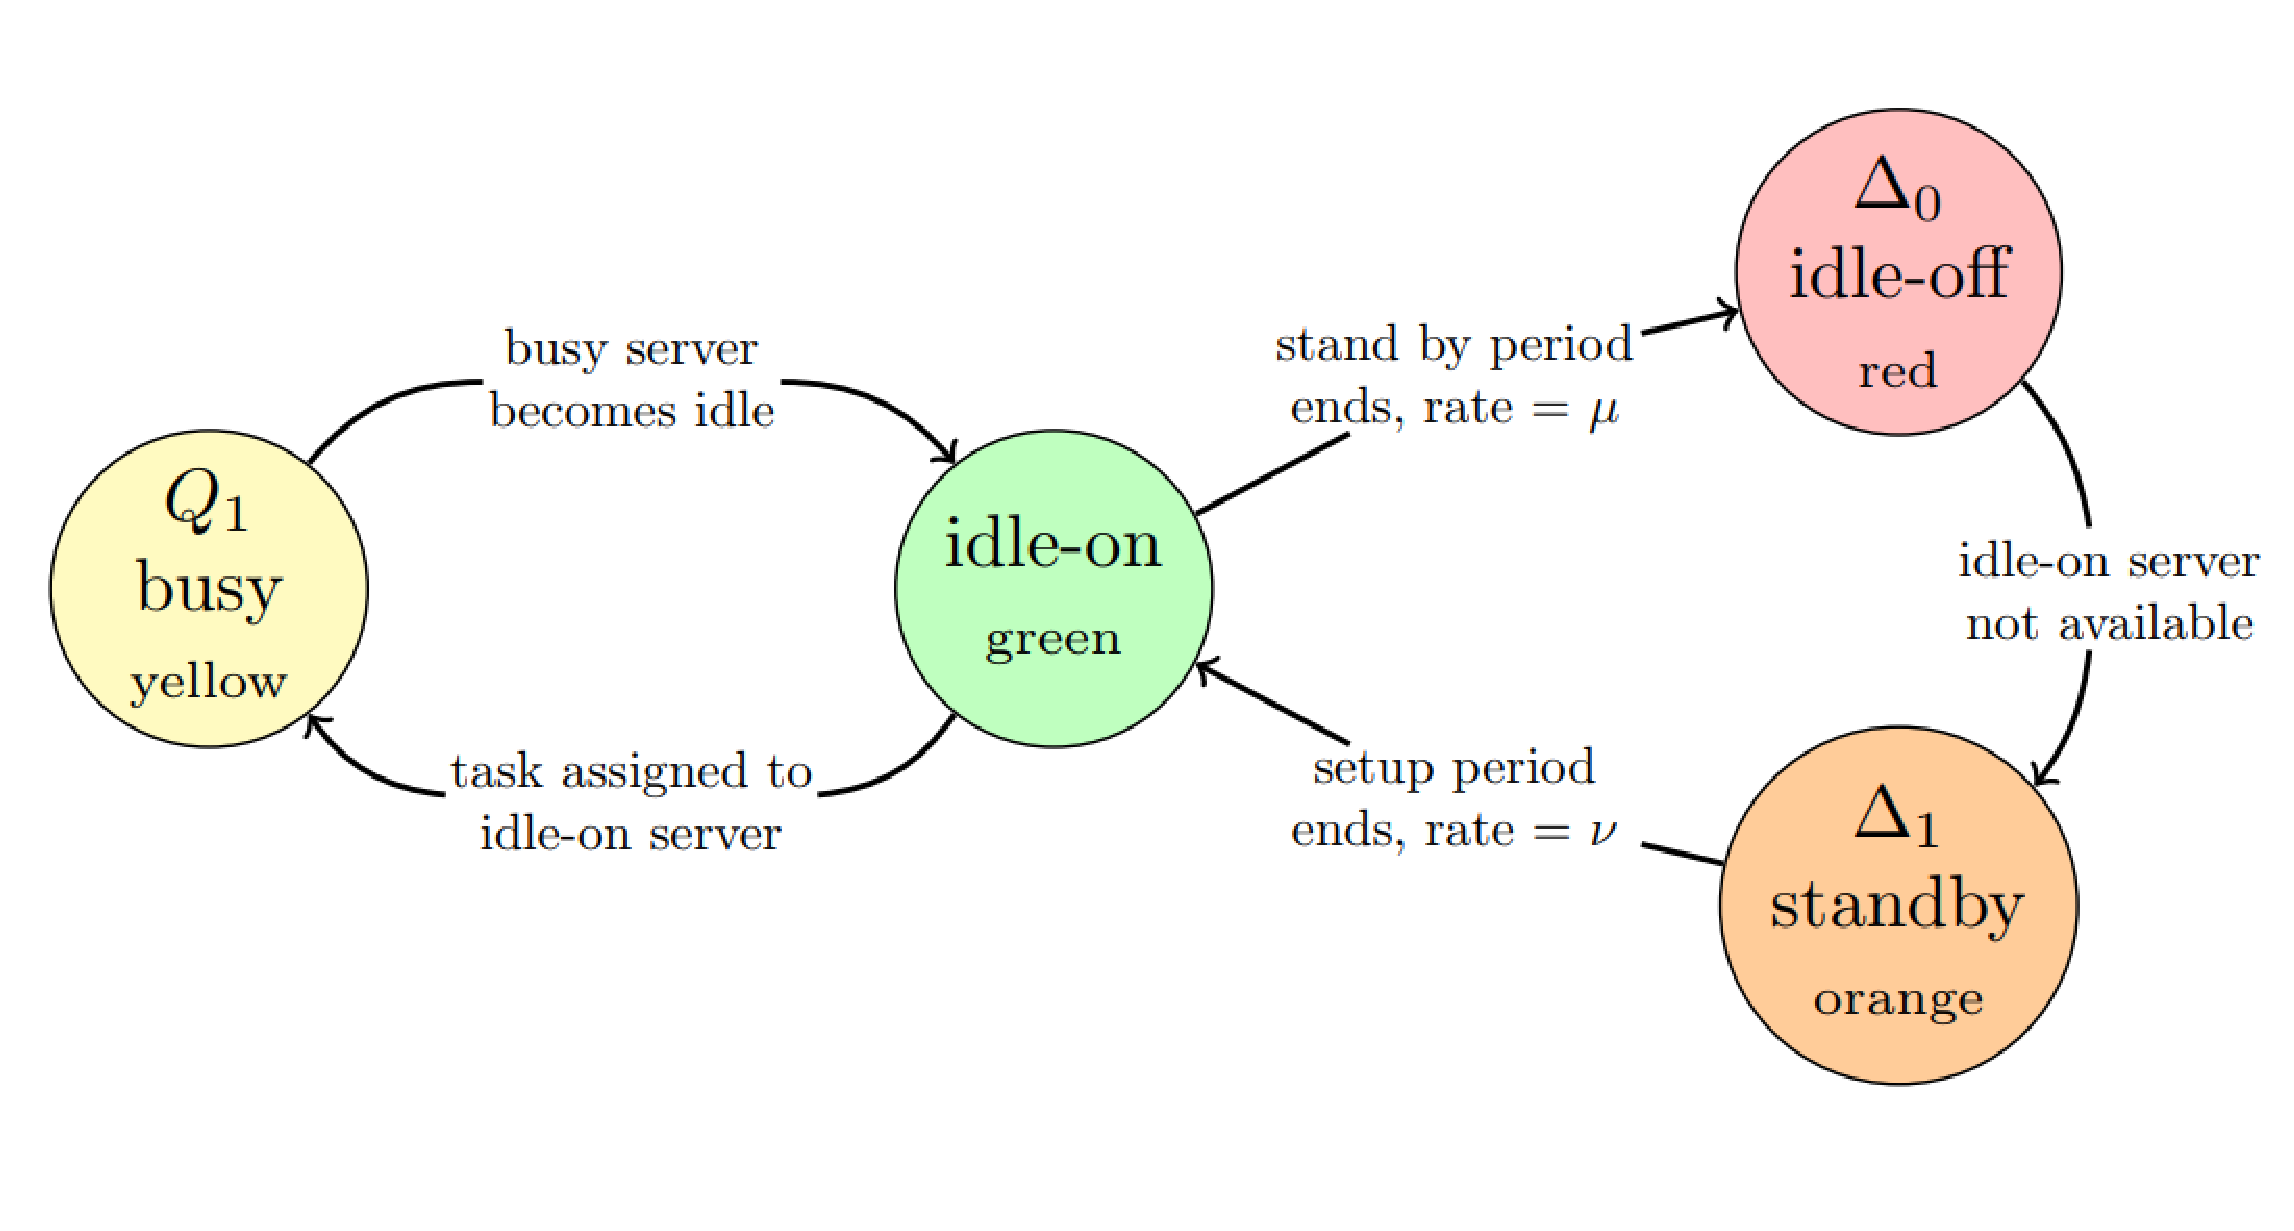
\includegraphics[scale=0.35]{imgs/tabs.eps}
    \caption{\label{fig:TABS}Server Decision flow as implemented in TABS.}
\end{figure*}

\noindent So from the perspective of the dispatcher, when a job arrives, the dispatcher will choose a random green server and forward the job
to that server. If there are not any green servers, then the dispatcher will choose a random yellow server and forward the job there. Then,
if there are any red servers, then the dispatcher will send a message to a random red server and tell it to turn on, at which point it will
enter a setup period $t_{setup}$ which follows the distribution $t_{setup} \sim Exp(\nu)$. It is worth noting that red and orange servers will
never be sent jobs, but green and yellow servers can be sent jobs (with affinity for the former), this is done to minimize job waiting time as
much as possible. It is also worth noting that the setup procedures are never aborted, even if green servers become available.


\noindent With the algorithm defined, we will now prove the asymptotic optimality of TABS; whereby both the mean waiting time and mean energy wastage
($\mathbb{E}[\textup{W}^N]$ and $\mathbb{E}[\textup{Z}^N]$, respectively) vanish as $N \rightarrow \infty$.


\pagebreak
\section{Proofs}

\subsection{Definitions}
\noindent \textbf{Given: } a distributed computing system with \textit{N} total servers, each with exponential service process;
\begin{center}
    $\left\{S(t)\right\}_{t\geq0} \sim Exp(\mu_{service})$,
\end{center}
and the Poisson arrival process;
\begin{center}
    $\left\{A(t)\right\}_{t\geq0} \sim Exp(N\lambda)$,
\end{center}
and buffer size $B = 1$, such that the overall system can be defined as an M/M/N/2N system, as seen in Figure \ref{fig:mmn2n};
\begin{figure*}[h]
    \centering
    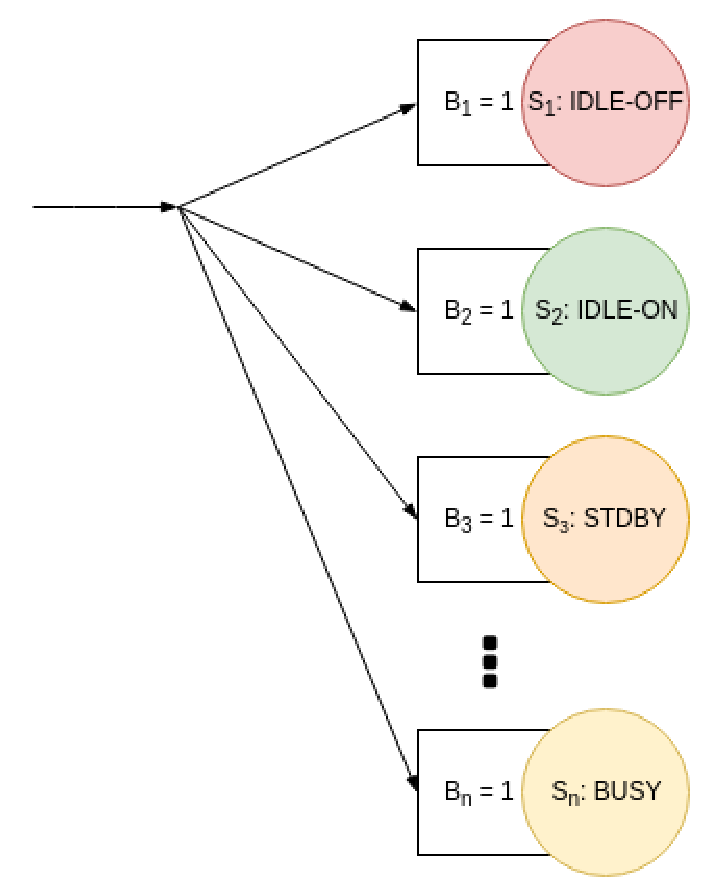
\includegraphics[scale=0.5]{imgs/M_M_N_2N.eps}
    \caption{\label{fig:mmn2n}An M/M/N/2N Server system with TABS.}
\end{figure*}
\newline\newline
\noindent \textbf{Define: }
\begin{equation} \label{eq:1}
    q_i^{(N)}(t) = \dfrac{Q_i^{(N)}(t)}{N}
\end{equation}
\begin{equation}\label{eq:2}
    \delta_0^{(N)}(t) = \dfrac{\Delta_0^{(N)}(t)}{N}
\end{equation}
\begin{equation}\label{eq:3}
    \delta_1^{(N)}(t) = \dfrac{\Delta_1^{(N)}(t)}{N}
\end{equation}



\noindent Where Eqn. \ref{eq:1} is the fraction of N servers that have at least \textit{i}
jobs queued at time \textit{t}, Eqn. \ref{eq:2} is the fraction of N servers that are in
idle-off mode at time \textit{t}, and Eqn. \ref{eq:3} is the fraction of N servers that
are in setup mode at time \textit{t}. Now we can say that the process $\left\{\textbf{Q}^N(t),\Delta_0^N(t),\Delta_1^N(t)\right\}_{t\geq0}$
fully describes the evolution of the system and is Markovian. However, the analysis of
such a process is extremely difficult due to the coupling between all the service processes,
and thus we resort instead to asymptotic analysis and consider the situation when $N \rightarrow \infty$,
and use the above quantities to define the following vector quantities;

\begin{equation} \label{eq:4}
    \textbf{q}^N(t) = \left(q_1^{(N)}(t),\ldots,q_B^{(N)}(t) \right)
\end{equation}
\begin{equation}\label{eq:5}
    \boldsymbol\delta^N(t) = \left(\delta_0^{(N)}(t), \delta_1^{(N)}(t) \right)
\end{equation}

\noindent Now, using Eqn. \ref{eq:4} and Eqn. \ref{eq:5}, we define \textbf{E};
\begin{equation}\label{eq:6}
    \textbf{E} = \left\{(\textbf{q},\boldsymbol\delta)\in[0,1]^{B+2} : q_i \geq q_{i+1},\forall i,\delta_0+\delta_1+\sum_{i=1}^B q_i \leq 1\right\}
\end{equation}

\noindent Eqn. \ref{eq:6} defines the space of all possible system states with
respect to time, such that $(\textbf{q}^N(t),\boldsymbol\delta^N(t))\in\textbf{E}, \forall t$.

\subsection{Fluid Limit for Exponential Service Distributions}

\noindent Here we will show that, in the case where $\lambda(t) \triangleq \lambda, \forall t$, the system state space \textbf{E} has a fixed point, and lead into the optimality proof.

\noindent \textbf{Assume that: }
\begin{equation}\label{eq:7}
    \left(\textbf{q}^N(0),\boldsymbol\delta^N(0)\right) \stackrel{d}{\rightarrow} \left(\textbf{q}^\infty,\boldsymbol\delta^\infty\right) \in \textbf{E}
\end{equation}\label{eq:7}

\noindent as $N\rightarrow\infty$. Then,
\begin{equation}
    \left\{\textbf{q}^N(t),\boldsymbol\delta^N(t)\right\}_{t\geq0} \stackrel{d}{\rightarrow} \left\{\textbf{q}(t),\boldsymbol\delta(t)\right\}_{t\geq0} \in \textbf{E}
\end{equation}

\noindent Note that the process $\left\{\textbf{q}(t),\boldsymbol\delta(t)\right\}_{t\geq0}$ is deterministic, and fully describes the system in the limit ($N \rightarrow \infty$). In \S3.1,
Mukherjee et al. derive several integral equations which describe the fluid limit of the system as described thus far. Please refer there for the derivation, as it is highly involved. The equations
are as follows:
\begin{equation}
    q_i(t) = q_i^\infty + \int_0^t \lambda(s)p_{i-1}(\textbf{q}(s),\boldsymbol\delta(s),\lambda(s))ds - \int_0^t (q_i(s)-q_{i+1}(s))ds, i = 1,\ldots,B
\end{equation}
\begin{equation}
    \delta_0(t) = \delta_0^\infty + \mu\int_0^t u(s)ds - \xi(t)
\end{equation}
\begin{equation}
    \delta_1(t) = \delta_1^\infty + \xi(t) - \nu\int_0^t \delta_1(s)ds
\end{equation}

\noindent where:
\begin{equation}
    u(t) = 1 - q_1(t) - \delta_0(t) - \delta_1(t)
\end{equation}
\begin{equation}
    \xi(t) = \int^t_0\lambda(s)(1-p_0(\textbf{q}(s),\boldsymbol\delta(s),\lambda(s0)))\mathbbm{1}_{\left[\delta_0(s)>0\right]}ds
\end{equation}
\noindent and for any $(\textbf{q},\boldsymbol\delta)\in \textbf{E}, \lambda>0$:
\begin{equation}
    p_0(\textbf{q},\boldsymbol\delta,\lambda) =
    \begin{cases}
        1,                                                              & \text{if $u = 1-q_1 -\delta_0 -\delta_1>0$}, \\
        \textup{min}\left\{\lambda^{-1}(\delta_1\nu+q_1-q_2),1\right\}, & \text{otherwise},                            \\
    \end{cases}
\end{equation}
\begin{equation}
    p_i(\textbf{q},\boldsymbol\delta,\lambda) = \left(1-p_0(\textbf{q},\boldsymbol\delta,\lambda)\right)\left(q_i-q_{i+1}\right)q_1^{-1}, i=1,\ldots,B
\end{equation}

\noindent Where $u(t)$ is the asymptotic fraction of unused resources at time \textit{t},
$\xi(t)$ is the asymptotic fraction of server setups started in the interval [0,\textit{t}],
$p_i(\textbf{q},\boldsymbol\delta,\lambda)$ is the instantaneous fraction of incoming jobs assigned to some server with queue length $q_i$
when the system state is $(\textbf{q},\boldsymbol\delta)$.
\subsection{Fixed Point in System State Space}
\noindent From these equations, we can derive that there is a fixed point within \textbf{E}, in the following location:
\begin{equation}
    \delta_0^*=1-\lambda,\qquad\delta_1^*=0,\qquad q_1^*=\lambda,\qquad q_i^*=0
\end{equation}
\noindent It is very important to note that these fixed point values are completely independent of the values $\nu$ and $\mu$.
This implies that for any values of $\nu$ and $\mu$, the system will always reach this equilibrium point as $t \rightarrow\infty$.
\subsection{Performance Metrics for $\mathbb{E}[Z^N]$}
\noindent We mentioned earlier that one of the quantities we wanted to optimize for was wasted energy ($\mathbb{E}[Z^N]$),
however we have not defined it. Let us first define $\mathbb{E}[P^N]$ to be the power usage of the $N^{th}$ server in the system.
Note that the power usage of an idle-on ("green") server is less than one which is starting up ("orange") or a busy one ("yellow"), while
an idle-off ("red") server uses 0 Watts. Let us then define $P_{full}$ to be the power used by orange and yellow servers,
and $P_{idle}$ to be the power used by green servers.
\footnote{Note that while yellow servers can be considered to be doing useful work (i.e. processing jobs), green servers can be seen
    as the primary source of wasted energy. This will be important during the proof.} In order for the system to be stable, at least a fraction
of the total servers $\lambda$ must be on in order to handle the incoming tasks. Thus, the lower bound on energy usage per server is $\lambda P_{full}$.
It follows naturally that we should define the wasted energy as the energy used minus the lower bound;
\begin{equation}
    \mathbb{E}[Z^N]=\mathbb{E}[P^N]-\lambda P_{full}
\end{equation}

\subsection{Proof of TABS Asymptotic Optimality - Waiting Time}
\begin{proof}{When $\lambda < 1$, for any $\mu > 0, \nu > 0$ as $N\rightarrow\infty:$}
    \begin{align*}
        \mathbb{E}[W^N] & = \dfrac{\mathbb{E}[L^N]}{N\lambda}, \textup{ where } \mathbb{E}[L^N] \triangleq \sum_{i=2}^BQ_i^N                     \\
        \mathbb{E}[W^N] & = \dfrac{\sum_{i=2}^BQ_i^N}{N\lambda}                                                                                  \\
        \mathbb{E}[W^N] & = \dfrac{\sum_{i=2}^Bq_i^N}{\lambda}                                                                                   \\
        \mathbb{E}[W^N] & = \dfrac{\sum_{i=2}^Bq_i^*}{N\lambda}, \textup{ where } q_i^* = 0, \forall i \geq 2 \textup{ as } N \rightarrow \infty \\
        \mathbb{E}[W^N] & \rightarrow 0 \textup{ as } N \rightarrow \infty
    \end{align*}

\end{proof}

\subsection{Proof of TABS Asymptotic Optimality - Wasted Energy}
\noindent First, let $U^N$ equal the number of idle-on servers:
\begin{equation*}
    U^N \triangleq N-Q_1^N-\Delta_0^N-\Delta_1^N
\end{equation*}

\begin{proof}{When $\lambda < 1$, for any $\mu > 0, \nu > 0$ as $N\rightarrow\infty:$}
    \begin{align*}
        \mathbb{E}[P^N] & = \dfrac{1}{N}\mathbb{E}\left[\left(Q_1^N+\Delta_1^N\right)P_{full} + U^NP_{idle}\right]                                                                  \\
        \mathbb{E}[P^N] & = \mathbb{E}\left[\left(q_1^N+\delta_1^N\right)P_{full} + u^NP_{idle}\right]                                                                              \\
        \mathbb{E}[P^N] & \rightarrow \left(q_1^*+\delta_1^*\right)P_{full} + u^*P_{idle} \textup{ where } q_1^* = \lambda, \delta_1^* = 0, u^* = 0 \textup{ as }N\rightarrow\infty \\
        \mathbb{E}[P^N] & \rightarrow \left(\lambda+0\right)P_{full} + 0P_{idle} \textup{ as }N\rightarrow\infty                                                                    \\
        \mathbb{E}[P^N] & \rightarrow \lambda P_{full} \textup{ as }N\rightarrow\infty                                                                                              \\
        \mathbb{E}[Z^N] & \triangleq \mathbb{E}[P^N] - \lambda P_{full}                                                                                                             \\
        \mathbb{E}[Z^N] & \rightarrow \lambda P_{full} - \lambda P_{full} \textup{ as }N\rightarrow\infty                                                                           \\
        \mathbb{E}[Z^N] & \rightarrow 0 \textup{ as }N\rightarrow\infty                                                                                                             \\
    \end{align*}

\end{proof}
\noindent Here we have proven the asymptotic optimality of TABS, both in terms of waiting time, and wasted energy.
These results can also be proven for the case of phase-type arrival distributions where $\lambda(t) \neq \lambda \forall t$,
which Mukherjee et. al prove as well.


\section{Simulation Results}
\noindent Mukherjee et al. corroborate their results with the following simulations:
\subsection{Convergence of Sample Paths to Fluid-Limit Trajectories}
\noindent The trajectories of the fluid limit quantities are analyzed under several arrival distributions
(i.e. Constant arrival rate, Sinusoidal arrival rate, and Hyperexponential arrival rate). The results
for the time-varied arrival scenario was most interesting, as it considered how TABS might perform in
a real-world computing system, where load will very rarely be constant, and can generally be modeled
by a sinusoidal process. Most notably, the resultant trajectories in the sinusoidal case show that the system's reactive
ability is immense, as the modeled arrival rate varies extremely quickly with respect to the mean service time,
yet the TABS scheme is able to balance the load extremely effectively.

\begin{figure*}[h]
    \centering
    \subfloat[My Results]{{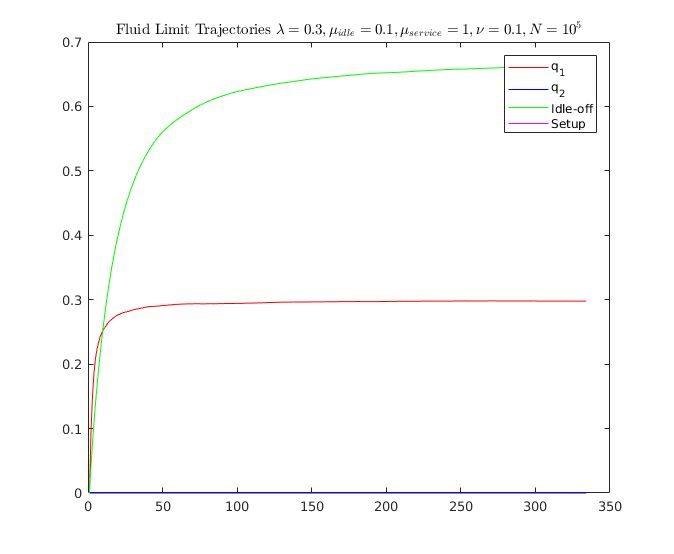
\includegraphics[width=.4\linewidth]{imgs/fluidLimitTrajectories.png} }}%
    \qquad
    \subfloat[Mukherjee et al.'s Results]{{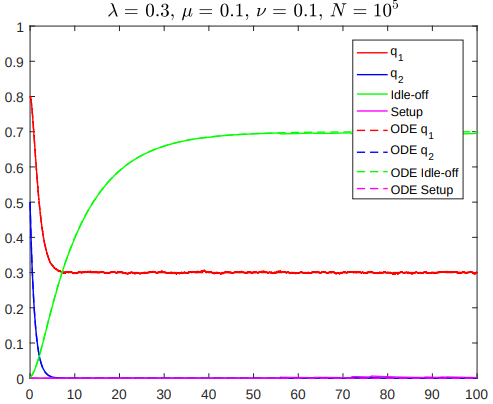
\includegraphics[width=.4\linewidth]{imgs/g1.png} }}%
    \caption{Fluid Limit Trajectories for constant arrival rate}%
    \label{fig:sims1}
\end{figure*}

\noindent In both the constant arrival and hyperexponential scenarios, the simulations illustrate that the TABS scheme
will always reach the fluid limit, regardless of the distribution of arrivals. I replicated the case where 
$\lambda(t) \triangleq \lambda = 0.3, \forall t$. My simulations (shown in figure \ref{fig:sims1}) the same asymptotic limits as Mukherjee et al.
yet the initial evolution of the system differs. This is due to the fact that my simulations assumed that the
entire system began as idle-on. I would say this is a meaningful comparison, because it shows through simulation
that the TABS scheme is entirely insensitive of initial conditions, and proves that there is a system-wide fixed point.


\begin{figure*}[h]
    \centering
    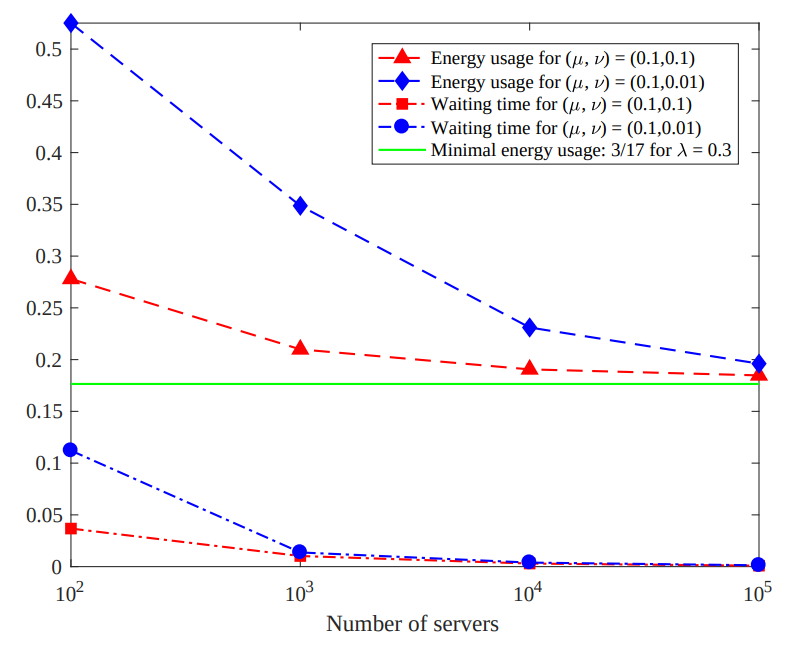
\includegraphics[width=.5\textwidth]{imgs/g2.png}
    \caption{\label{fig:waitingtime_lostenergy}Convergence of $\mathbb{E}[W^N] \textup{ and }\mathbb{E}[Z^N]$ under TABS for various values of \textit{N}}
\end{figure*}

\subsection{Convergence of Steady-State Performance Metrics to Fluid-Limit Values}
\noindent Mukherjee et al. also show that the performance metrics (i.e. Waiting Time and Wasted Energy)
vanish in the limit as $N\rightarrow\infty$. They show notably that this convergence occurs for different 
values of $\mu$ and $\nu$, however the rate of convergence for $\mathbb{E}[Z^N]$ is severely effected for
small values of $\nu$, as seen in Figure \ref{fig:waitingtime_lostenergy}.


\section{Further Work}
\noindent While this is a phenomenal and comprehensive work, there are several extensions that I could see being explored. I would be very interested in
combining this scheme with a Power-of-d choices type algorithm for finding the best green or yellow server to use. I believe that there could be significant
improvement in latency, but the additional overhead of calculating these choices negates the benefit of not having to retain global queue information, however since
we only need to keep queue information for d yellow servers at each time, and eventually the yellow servers will vanish in the limit, then application of power-of-d
should help this scheme to converge faster. However, this is mere speculation and I have no simulations yet to corroborate my hypothesis. If I am able to find the time,
I will definitely be exploring this extension. 

\end{document}
